\documentclass[tikz,border=2pt]{standalone}
\usepackage{amsmath,amssymb}
\usepackage{pgfplots}
\pgfplotsset{compat=1.18}

\begin{document}
% Joint density 2 on the triangle 0 < x < y < 1. Fixing Y = y cuts a horizontal slice of length y;
% rescaling the slice by f_Y(y) = 2y gives the conditional density 1/y on (0, y).
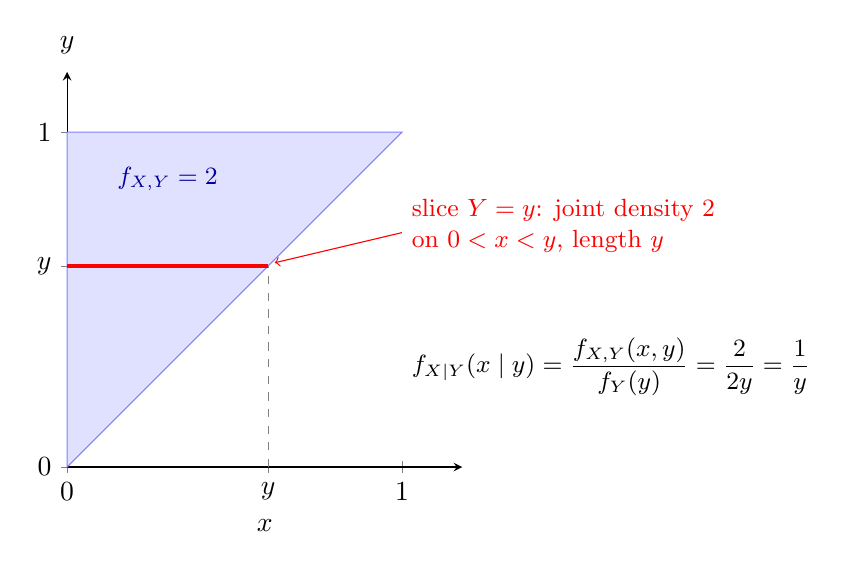
\begin{tikzpicture}
	\begin{axis}[
		axis lines=left, xmin=0, xmax=1.18, ymin=0, ymax=1.18,
		xtick={0,0.6,1}, xticklabels={$0$,$y$,$1$}, ytick={0,0.6,1}, yticklabels={$0$,$y$,$1$},
		xlabel={$x$}, ylabel={$y$}, ylabel style={rotate=-90, anchor=south, at={(axis description cs:0,1.02)}},
		width=6.6cm, height=6.6cm, clip=false
		]
		\addplot[fill=blue!12, draw=blue!50] coordinates {(0,0) (1,1) (0,1)} -- cycle;
		\draw[red, very thick] (axis cs:0,0.6) -- (axis cs:0.6,0.6);
		\draw[gray, dashed] (axis cs:0.6,0) -- (axis cs:0.6,0.6);
		\node[blue!60!black, font=\small] at (axis cs:0.3,0.86) {$f_{X,Y}=2$};
		\node[red, anchor=west, font=\small, align=left] at (axis cs:1.0,0.72) {slice $Y=y$: joint density $2$\\ on $0<x<y$, length $y$};
		\draw[red, ->] (axis cs:1.0,0.7) -- (axis cs:0.62,0.61);
		\node[anchor=west, font=\small, align=left] at (axis cs:1.0,0.3) {$f_{X\mid Y}(x\mid y)=\dfrac{f_{X,Y}(x,y)}{f_Y(y)}=\dfrac{2}{2y}=\dfrac1y$};
	\end{axis}
	
\end{tikzpicture}
\end{document}
